\documentclass{article}
\usepackage[margin=1in]{geometry}
\usepackage{graphicx}
\usepackage{hyperref}
\usepackage{natbib}
\usepackage{soul}
\bibliographystyle{apalike}
\usepackage{amsmath}

\title{Supplementary Material \\ \large{Fish from the Sky: Airborne eDNA Tracks Aquatic Life}}

%\author{Yin Cheong Aden Ip$^1$\textbf{*} \and
%Gledis Guri$^1$\textbf{*} \and
%Elizabeth Andruszkiewicz Allan$^1$ \and
%Ryan P. Kelly$^1$}

\date{\today}

\begin{document}

\maketitle



\clearpage
\begin{figure}[tbhp] 
\centering
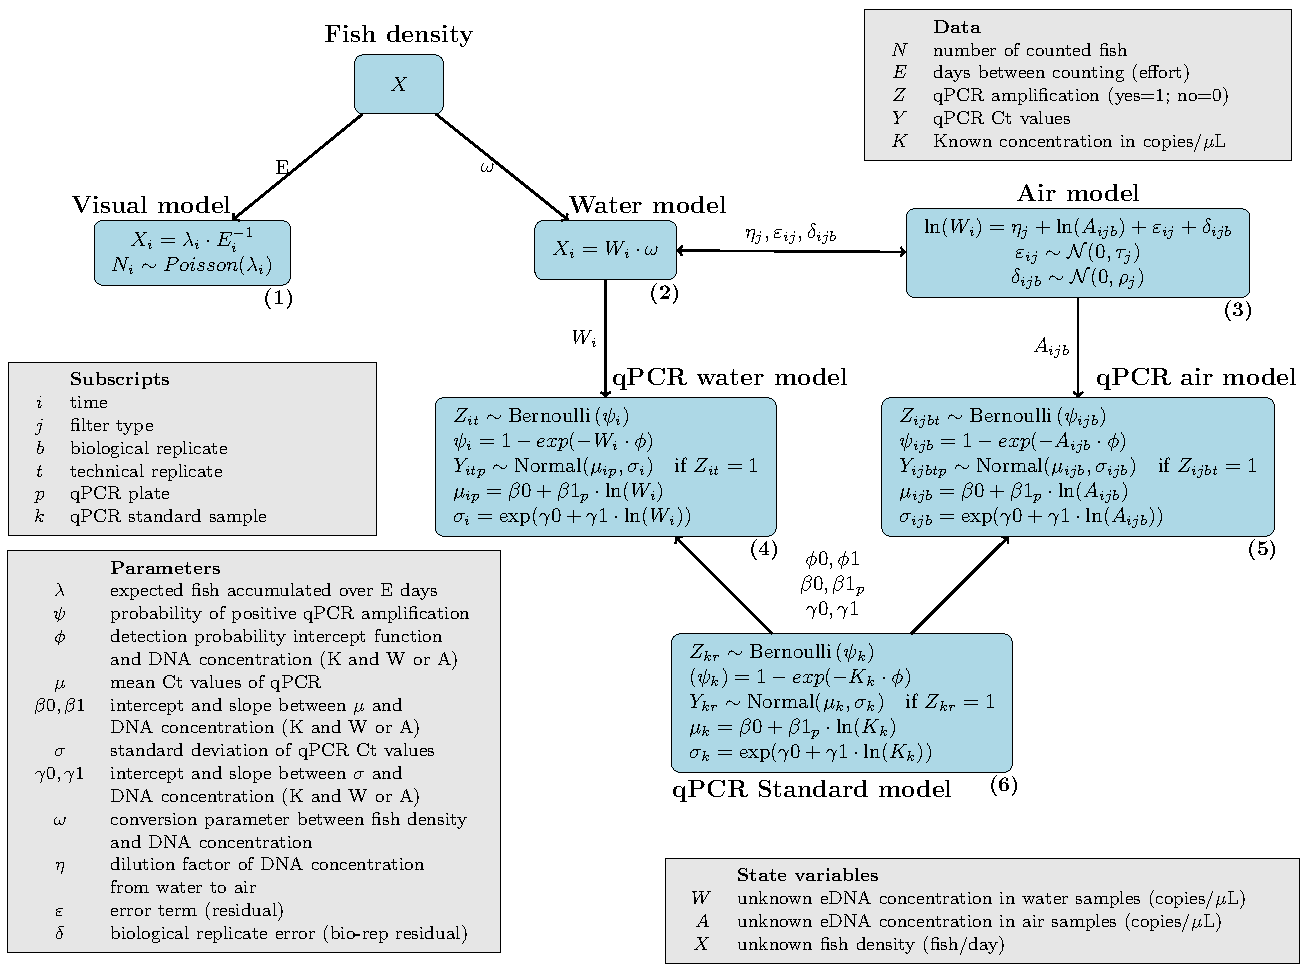
\includegraphics[width=16.5cm]{Plots/DAG.pdf}  
\caption{Directed acyclic graph (DAG) of joint Bayesian model for linking salmon migration dynamics from visual observation, water and air eDNA concentration.}
\label{fig:DAG}
\end{figure}

%Figure S2 -------------------- 

\begin{figure}[tbhp] 
\centering
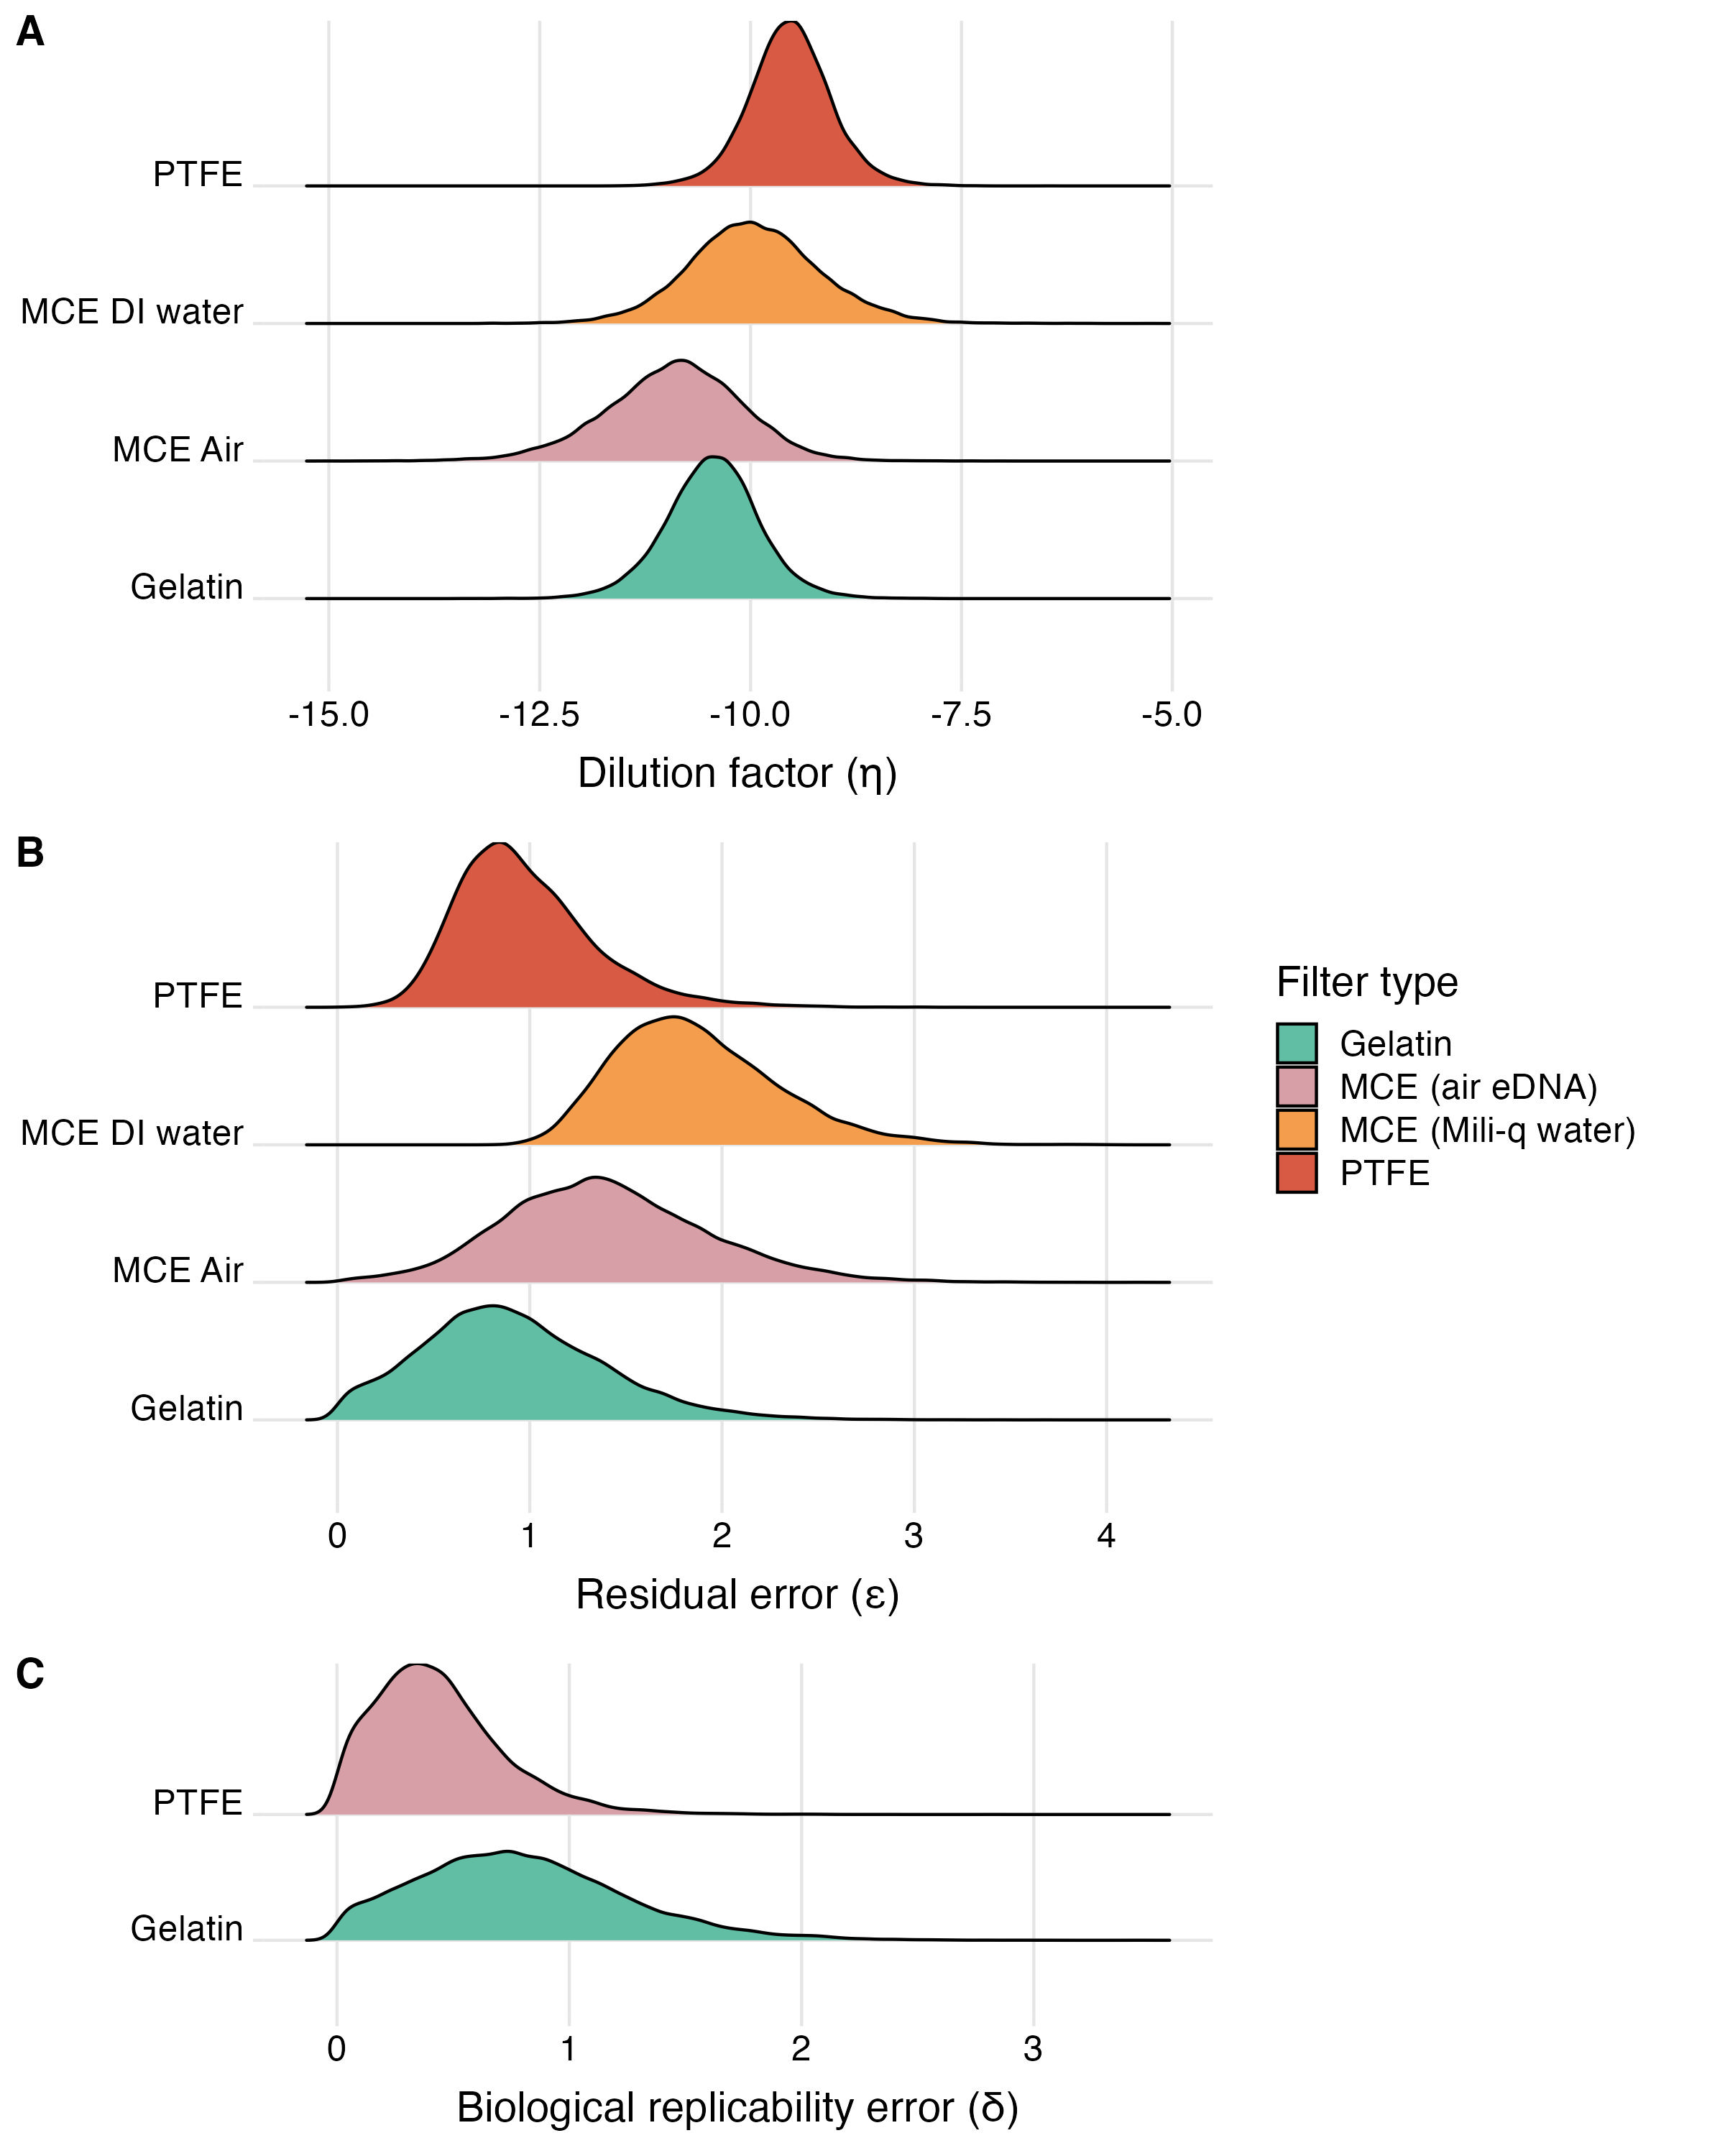
\includegraphics[width=15.5cm]{Plots/Figure_2.jpg}  
\caption{Density plots showing posterior distributions of: (A) water-to-air dilution factors ($\eta$), illustrating the magnitude of concentration reduction between aquatic and atmospheric matrices; (B) standard deviation (SD) of the residual error values ($\tau$), representing the congruence (lower = better) between estimated eDNA concentrations between air and water; and (C) standard deviation (SD) of the biological replicability error ($\rho$), quantifying measurement consistency (lower = better) between 
technical replicates of two air filters (PTFE and gelatin filters). Each parameter is estimated for each of four different air eDNA collection methods (differentiated by colors).}
\label{fig:fig2}
\end{figure}

%Figure S3 -------------------- 

\clearpage
\begin{figure}[tbhp] 
\centering
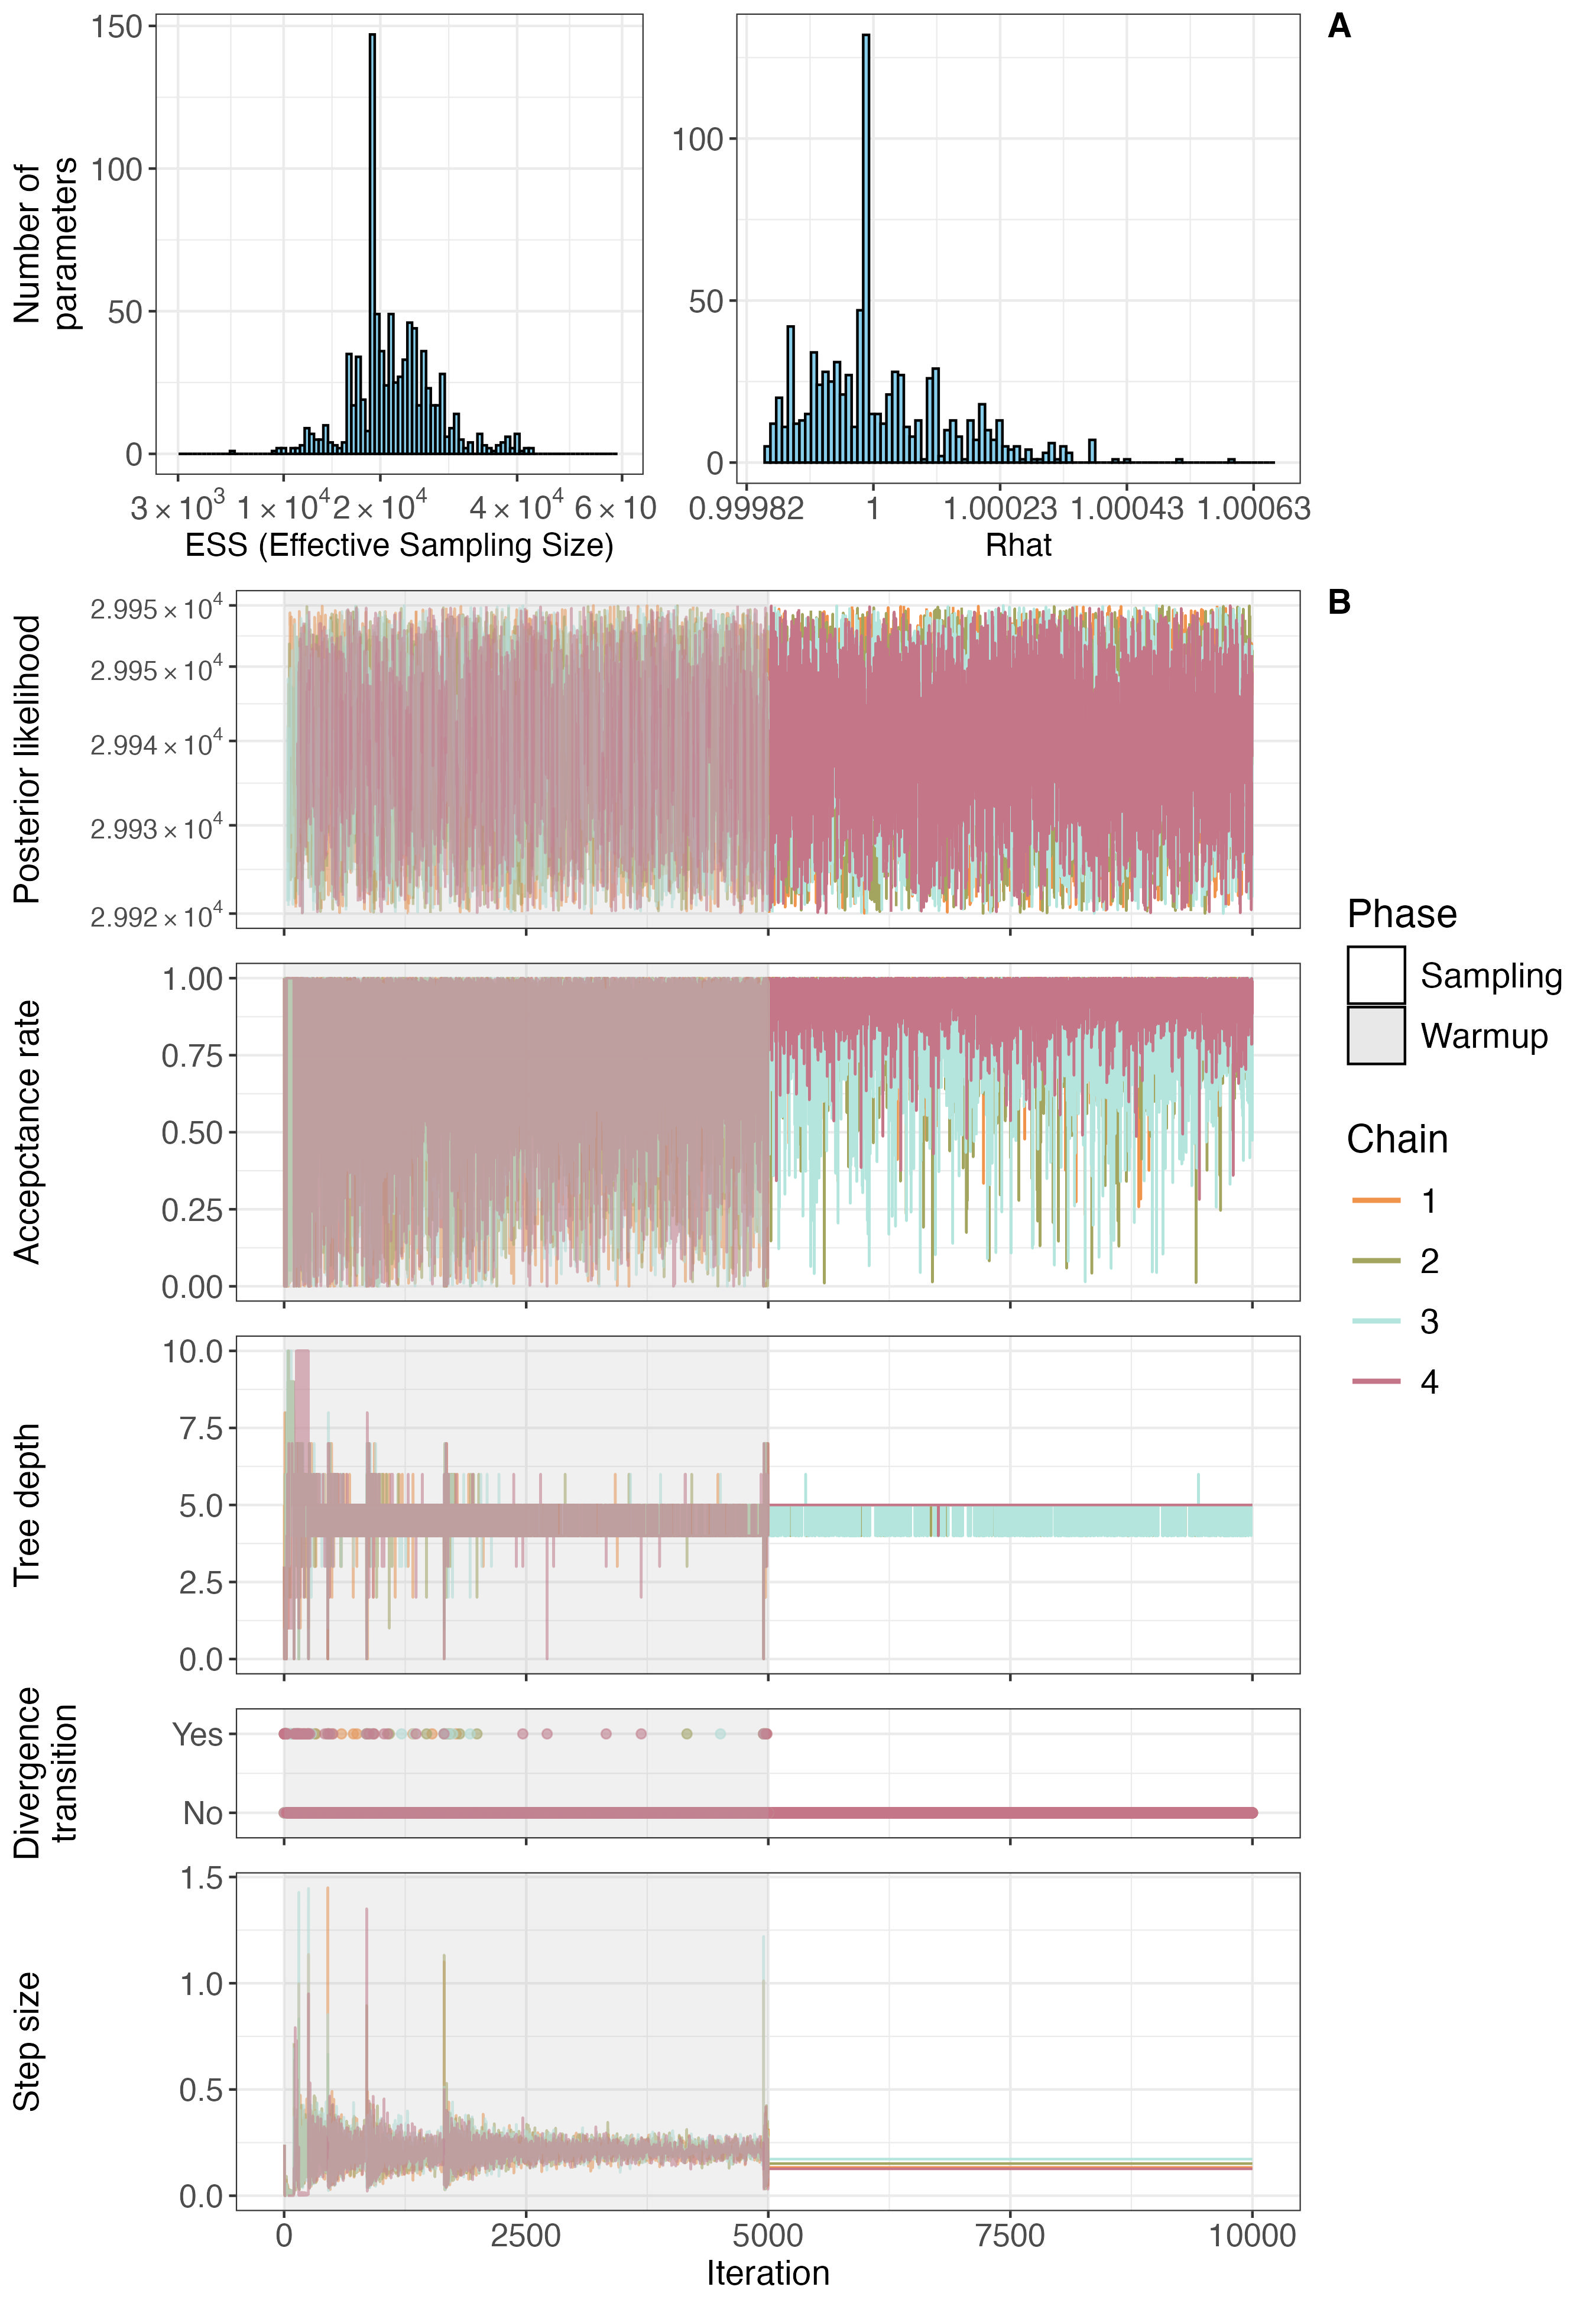
\includegraphics[width=14.2cm]{Plots/Diagnostic_Fig_1.jpg}  
\caption{Bayesian model convergence diagnostics indicating (A) the distributions of effective sample size (ESS, left) and $\hat{R}$ values (right) for all parameters and (B) convergence metrics across iterations, including posterior likelihood, acceptance rate, tree depth, divergence transitions, and step size for four MCMC chains. Warmup and sampling phases are distinguished by background shading.}
\label{fig:diagnostics}
\end{figure}

%Figure S4 -------------------- 

\clearpage
\begin{figure}[tbhp] 
\centering
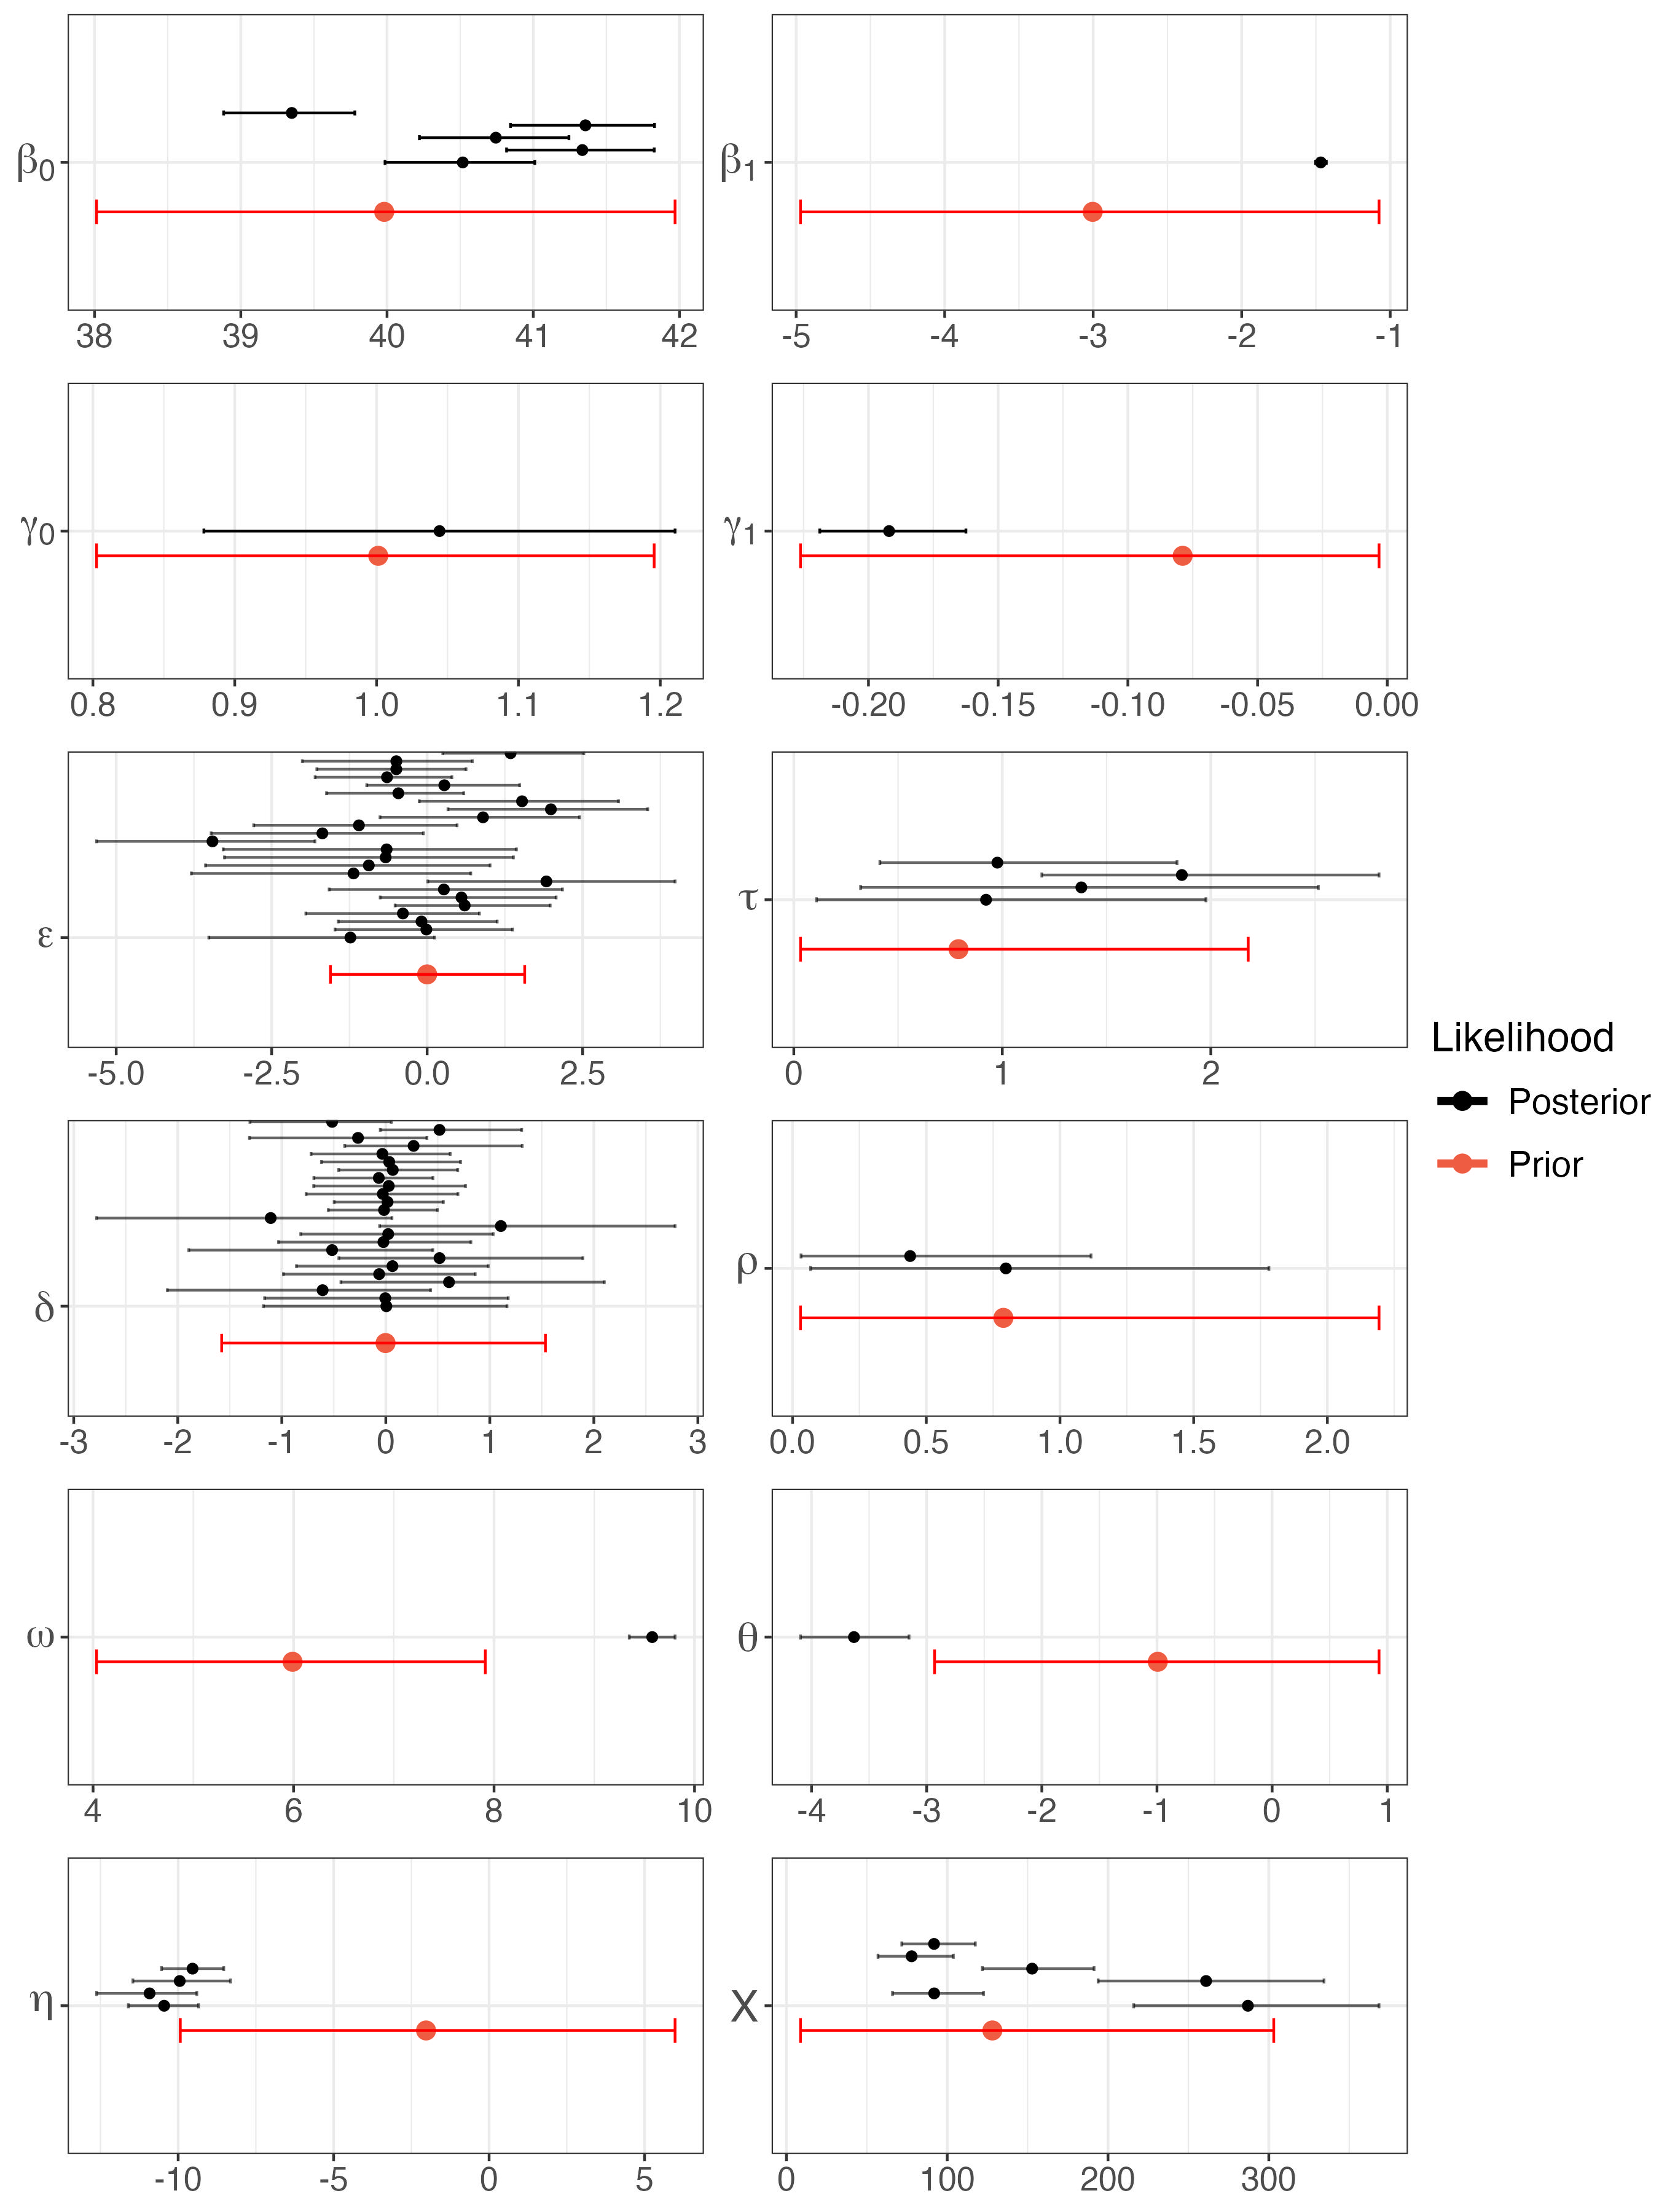
\includegraphics[width=15.5cm]{Plots/Diagnostic_Fig_2.jpg}  
\caption{Prior sensitivity analysis for model parameters ($\beta_0, \beta_1,, 
\gamma_0,\gamma_1,\varepsilon,\tau,\delta,\rho,\omega,\theta,\eta,X$). Black points and intervals represent posterior means and 95\% confidence intervals respectively and red points and intervals show prior mean and 95\% confidence intervals respectively.}
\label{fig:prior_sens}
\end{figure}


%Figure S5 -------------------- 

\clearpage
\begin{figure}[tbhp] 
\centering
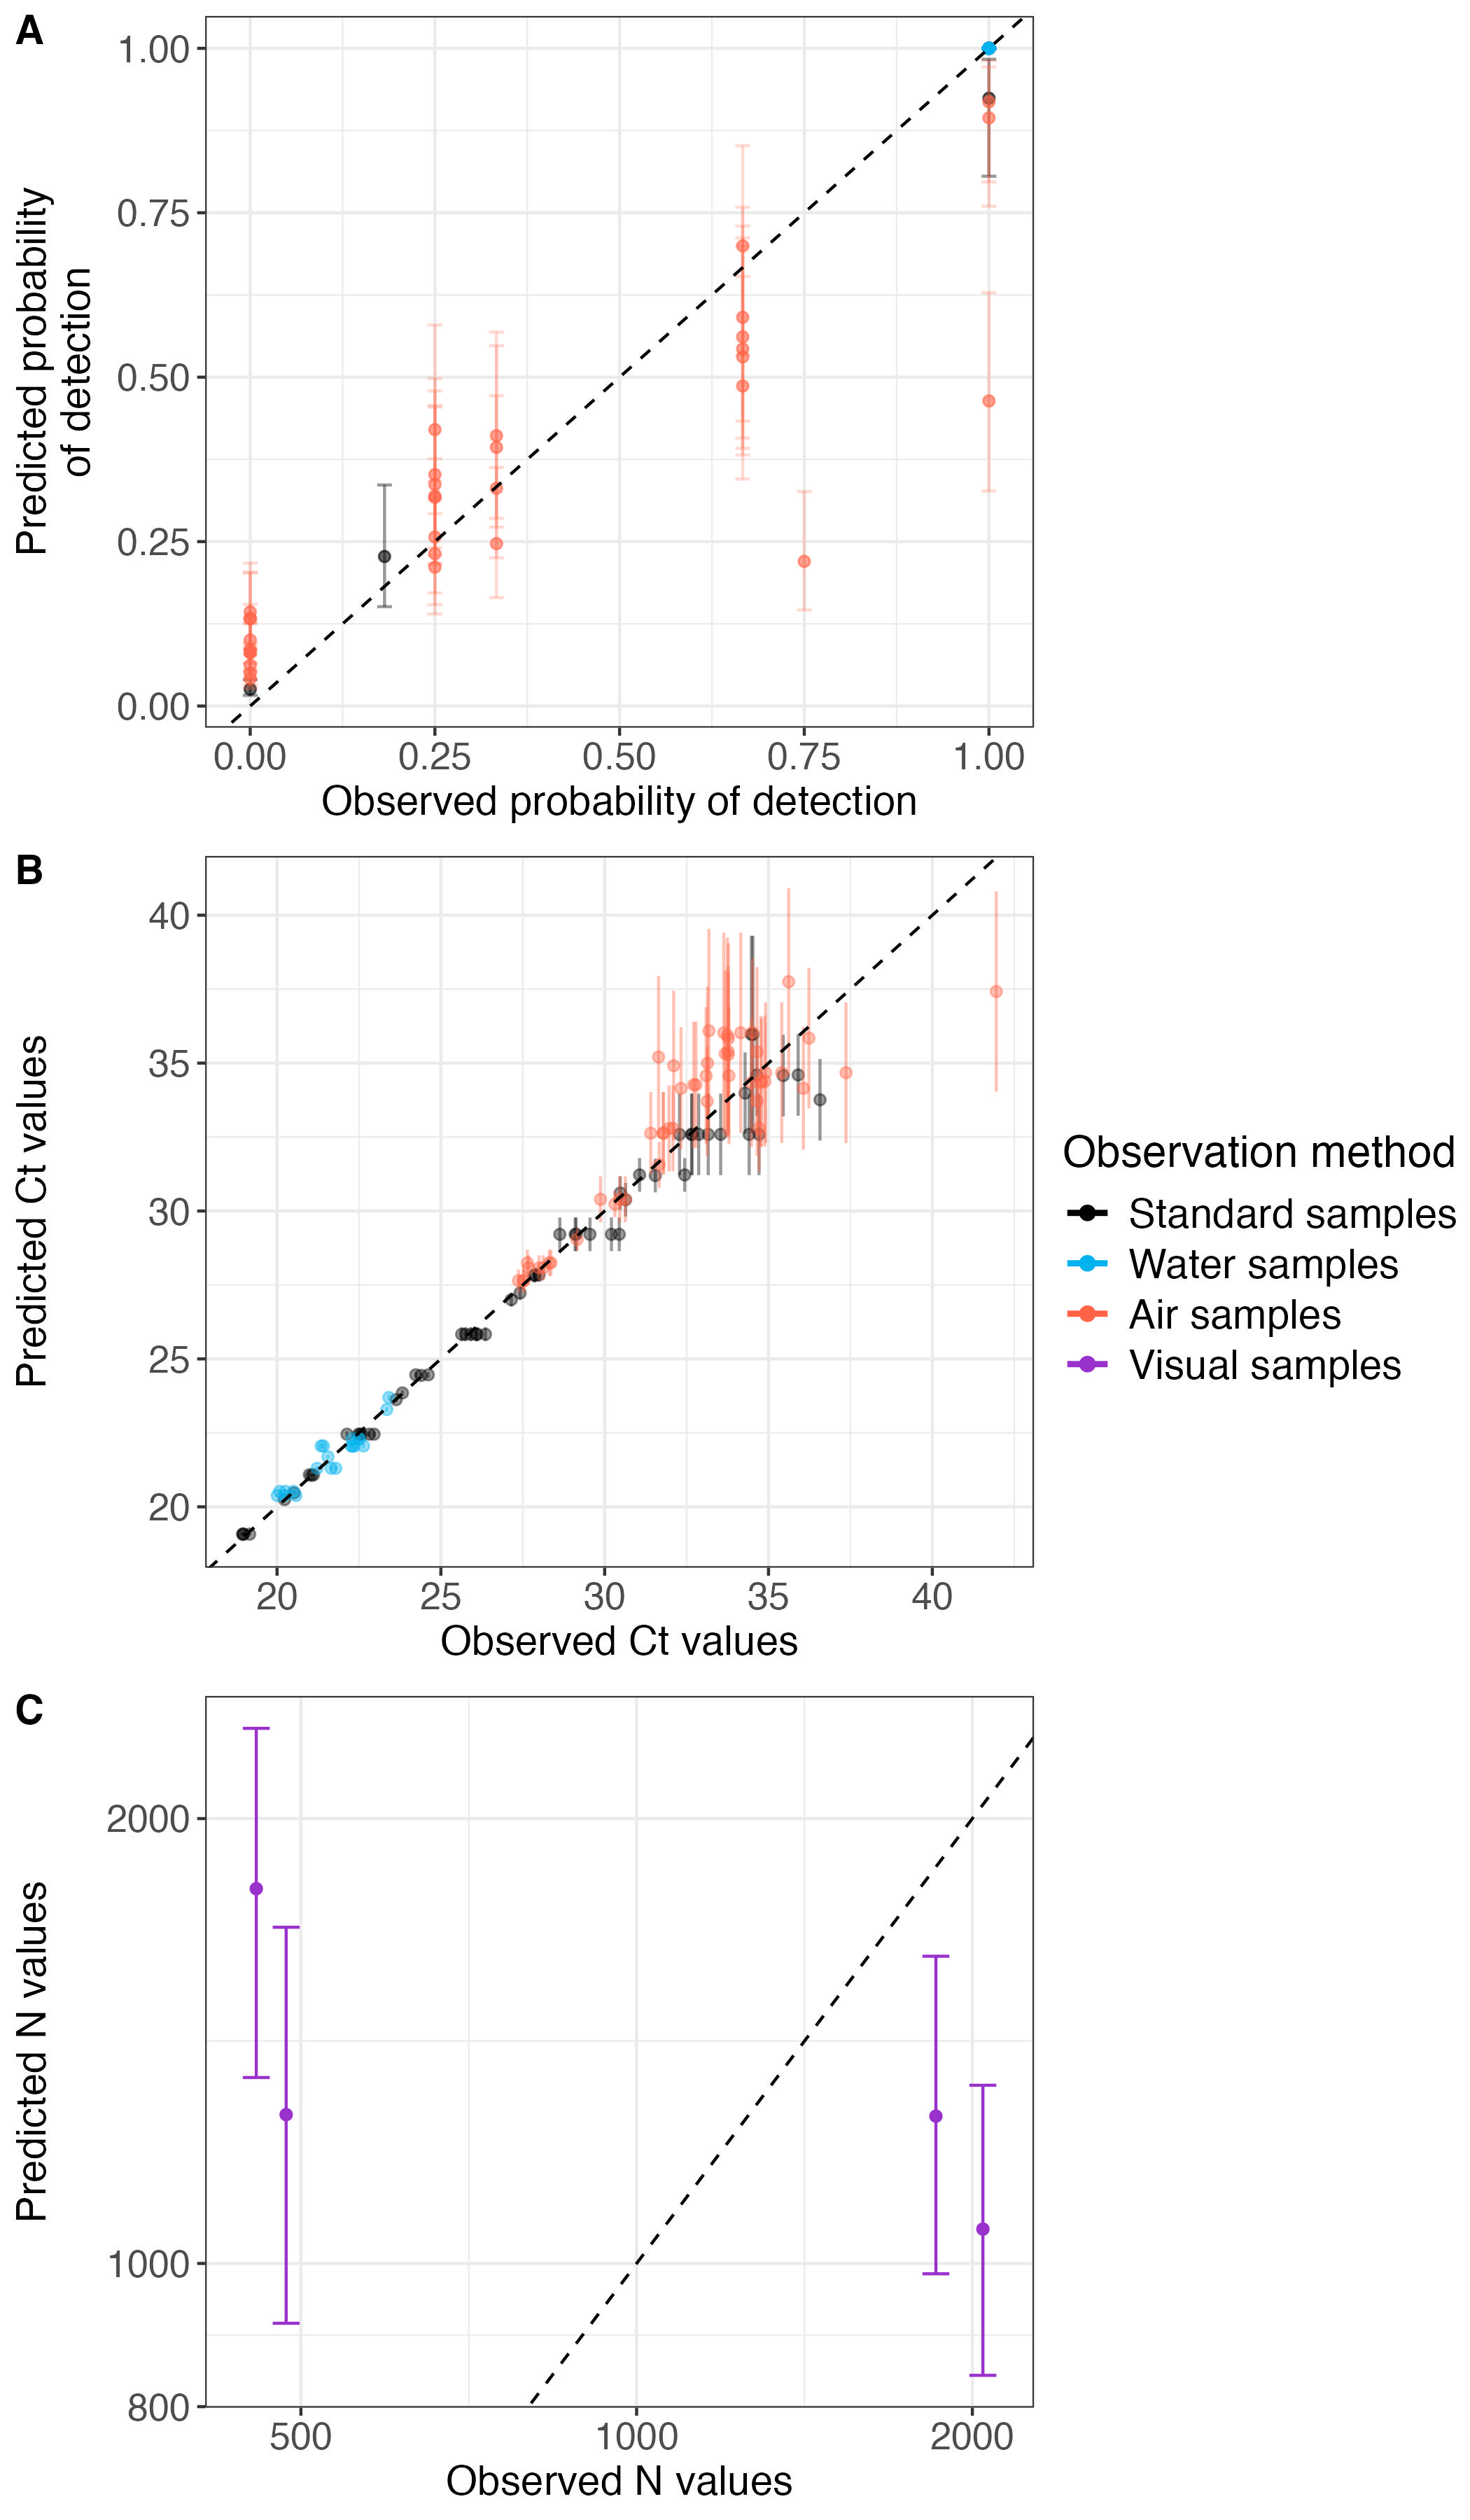
\includegraphics[width=12.0cm]{Plots/Diagnostic_Fig_3.jpg}  
\caption{Posterior predictive checks comparing observed vs. model-predicted values for (A) detection probability of air and water samples alongside standard samples, (B) Ct values for air and water samples alongside standard, and (C) visual counts of fish (N).}
\label{fig:postpred}
\end{figure}




%Table -------------------- 
\clearpage
\begin{table}
    \centering
    \begin{tabular}{lll}
         & \textbf{Description} & \textbf{Prior} \\
&Data & \\
\hline
$N$ & number of fish counted & - \\
$E$ & elapsed days between counting & - \\
$Z$ & qPCR amplification (yes=1; no=0) & - \\
$Y$ & qPCR cycle threshold (Ct) & - \\
$K$ & known DNA concentration (qPCR standards) & - \\
$V$ & Reaction volume in $\mu$L & - \\
$S$ & Surface area of air collection method cm/$^2$ & - \\

&&\\
&State processes&\\
\hline
$X$ & unknown fish density in (fish $\cdot$ day$^{-1}$) & $\mathcal{TN}(100,100;0,+\infty)$ \\
$W$ & unknown DNA concentration in water in (copies/L) & - \\
$U$&unknown eDNA concentration in water samples (copies/$\mu$L) & - \\
$A$ & unknown DNA concentration in air in (copies/day/cm$^2$) & - \\
$Q$ & unknown eDNA concentration in air samples (copies/$\mu$L) & - \\

&&\\

&Transformed parameters&\\
\hline
$\lambda$& expected fish accumulated over E days & - \\
$\psi$& probability of positive qPCR amplification & - \\
$\mu$& mean Ct values of qPCR & - \\
$\sigma$& standard deviation of qPCR Ct values & - \\
&&\\

&Fixed parameters&\\
\hline
$\phi$& overdispersion parameter of Negative Binomial & - ($\phi = 20$) \\
&&\\

&Parameters&\\
\hline
$\omega$& conversion parameter between fish density
and DNA concentration & $\mathcal{N}(6,1)$\\
$\eta$& dilution factor of DNA concentration
from water to air & $\mathcal{N}(-2,4)$\\
$\varepsilon$& time ($t$) specific error term (residual) & $\mathcal{N}(0,\tau)$\\
$\tau$& standard deviation of residuals & $\mathcal{TN}(0,1;0, +\infty)$\\
$\delta$& biological replicate error term (residual) & $\mathcal{N}(0,\rho)$\\
$\rho$& standard deviation of biological replicate error & $\mathcal{TN}(0,1;0, +\infty)$\\
$\theta$& intercept of the qPCR probability of detection ($\psi$) relationship &$\mathcal{N}(-1,1)$\\
& and eDNA concentration ($K$, $W$, and $A$) \\
$\beta0$& intercept of the linear relation between the mean Ct values ($\mu$)&$\mathcal{N}(40,1)$\\
&and eDNA concentration ($K$, $W$, and $A$) & \\
$\beta1$& slope of the linear relation between the mean Ct values ($\mu$) and &$\mathcal{N}(-3,1)$\\
&eDNA concentration ($K$, $W$, and $A$)) & \\
$\gamma0$& intercept of the linear relation between the standard deviation&$\mathcal{N}(1,0.1)$\\
&of Ct values ($\sigma$) and eDNA concentration ($K$, $W$, and $A$) & \\
$\gamma1$& intercept of the linear relation between the standard deviation &$\mathcal{N}(0,0.1)$\\
&of Ct values ($\sigma$) and eDNA concentration ($K$, $W$, and $A$) & \\
&&\\
&Index&\\
\hline
$t$& time (days) & -\\
$j$& filter type & -\\
$b$& biological sample replicate & -\\
$p$& qPCR plate & -\\
$k$& qPCR standard sample & -\\
$r$& qPCR technical replicate & -\\


    \end{tabular}
    \caption{Data, state processes, parameters, transformed parameters, and subscripts employed in the joint Bayesian model and their prior distributions}
    \label{tab:priortable}
\end{table}

\end{document}

